\documentclass[portuguese]{sbc2025}%

%\usepackage{graphicx}% já está incluido na classe
%\usepackage[utf8]{inputenc} % obsoleto, desnecessário

\usepackage[misc,geometry]{ifsym} 

%%%%  %\usepackage{fontspec}

%% Os problemas com a classe eram originados por carregarem ambos os
%% pacotes fontenc e fontspec simultaneamente. Agora a classe detecta
%% qual engine está em uso e se for o pdflates então carrega o
%% fontenc. Se forem o xelatex ou lualatex então carrega o
%% fontspec. Eu particularemnte prefiro o lualatex ou o xetex


% \usepackage{fontawesome} %%% incluido na classe. Desnecessário
% chamá-lo aqui


%%%% \usepackage{academicons}
%%%% outro encrenqueiro que se tornou desnecessario. Deste typeface só
%%%% se usava o glifo do orcid e o codigo interno bombava.
%%%% Substitui pelo pacote orcidlink (carregado internamete na classe)
%%%% e consertei o codigo na classe.


%\usepackage{color} % carregada dentro da classe
%\usepackage{hyperref} % carregada dentro da classe

\usepackage{aas_macros}
\usepackage[bottom]{footmisc}

%\usepackage{supertabular}
%\usepackage{multicol}
%\usepackage{multirow}
%% O pacote tabularray é muito melhor para
% a criacao de tabela complexas e/ou loooongas; tudo de modo simples.
%% Torna o uso de multicol e multirow desnecessarios

\usepackage{tabularray}


\usepackage{afterpage}
\usepackage{url}
\usepackage{pifont}


\setcitestyle{square}


\definecolor{engtitle}{rgb}{0.5,0.5,0.5}
\definecolor{orcidlogo}{rgb}{0.37,0.48,0.13}
\definecolor{unilogo}{rgb}{0.16, 0.26, 0.58}
\definecolor{maillogo}{rgb}{0.58, 0.16, 0.26}
\definecolor{darkblue}{rgb}{0.0,0.0,0.0}
\hypersetup{colorlinks,breaklinks,
            linkcolor=darkblue,urlcolor=darkblue,
            anchorcolor=darkblue,citecolor=darkblue}
%\hypersetup{colorlinks,citecolor=blue,linkcolor=blue,urlcolor=blue}

%%%%%%% IMPORTANT: We disable hyperlinks by default with this line, to avoid the error "\pdfendlink ended up in different nesting level" while writing.
%\hypersetup{draft}

\jid{REIC}
\jtitle{Revista Eletrônica de Iniciação Científica em Computação, 202X, XX:1}
\issn{3085-8461}
\doi{10.5753/reic.202X.XXXXXX}
\copyrightstatement{This work is licensed under a Creative Commons Attribution 4.0 International License}
\jyear{202X}

\category{Artigo de Pesquisa/Research Paper}
\title[Plataforma Web com Inteligência Artificial para Identificação de Doenças em Plantas]{Plataforma Web com Inteligência Artificial para Identificação de Doenças em Plantas}
\engtitle{\textcolor{engtitle}{Web platform with Artificial Intelligence for identifying plant diseases}}

%THE ORCID IS MANDATORY FOR EACH AUTHOR IN JBCS
\author[Quaresma em 2026]{
\affil{\textbf{Maria Quaresma}~\orcidlink{0000-0002-0339-6624}~\textcolor{blue}{\faEnvelopeO}~~[{Centro Federal de Educação Tecnologica Celso Sucknow da Fonseca}~|\href{mailto:maria.rocha@aluno.cefet-rj.br}{~{\textit{maria.rocha@aluno.cefet-rj.br}}}~]}

\affil{\textbf{Neemias Cruz}~\orcidlink{0000-0002-7110-2026}~\textcolor{blue}{\faEnvelopeO}~~[{Centro Federal de Educação Tecnologica Celso Sucknow da Fonseca}~|\href{mailto:neemiascruz@hotmail.com}{{\textit{neemiascruz@hotmail.com}}}~]}

}

\begin{document}

\begin{frontmatter}

\maketitle

\begin{mail}
Centro Federal de Educação Tecnologica Celso Sucknow da Fonseca, R. Miguel Ângelo, 96 - Maria da Graça, Rio de Janeiro - RJ, 20785-220, Brasil. 
\end{mail}


\begin{abstract-pt}
Este trabalho apresenta o desenvolvimento de uma plataforma web baseada em Inteligência Artificial para a identificação de doenças em
plantas por meio da análise de imagens de folhas. A solução foi implementada em arquitetura cliente-servidor, utilizando FastAPI,
JavaScript, PostgreSQL e Docker, e integra dois modelos de aprendizado profundo baseados na EfficientNetB0, responsáveis pela 
identificação da espécie vegetal e da doença associada. Os modelos foram treinados com imagens da base PlantVillage, utilizando uma 
abordagem de divisão hold-out entre conjuntos de treinamento e validação, visando aumentar a consistência dos diagnósticos. Além disso,
a plataforma oferece autenticação de usuários, armazenamento do histórico de análises e geração automática de informações textuais 
complementares. Os resultados demonstraram a viabilidade da abordagem proposta, evidenciando seu potencial de aplicação no contexto
da agricultura digital e do diagnóstico fitossanitário.

\end{abstract-pt}

\begin{abstract-en}
This work presents the development of a web platform based on Artificial Intelligence for the identification of plant diseases 
through the analysis of leaf images. The solution was implemented in a client-server architecture, using FastAPI, JavaScript, 
PostgreSQL, and Docker, and integrates two deep learning models based on EfficientNetB0, responsible for identifying the plant 
species and the associated disease. The models were trained with images from the PlantVillage database, using a hold-out split
approach between training and validation sets, increasing the consistency of diagnoses. In addition, the 
platform offers user authentication, storage of analysis history, and automatic generation of complementary textual 
information. The results demonstrated the viability of the proposed approach, highlighting its potential application in the 
context of digital agriculture and phytosanitary diagnosis.
\end{abstract-en}

\begin{pchaves}
Visão Computacional, Aprendizado Profundo, Agricultura Digital
\end{pchaves}

\begin{keywords}
Computer Vision, Deep Learning, Digital Agriculture
\end{keywords}

\begin{dates}
% This information will be provided by the editor before publishing the paper
\noindent{\sffamily\textbf{Recebido/Received:}} DD Month YYYY~~~$\bullet$~~~
{\sffamily\textbf{Aceito/Accepted:}} DD Month YYYY~~~$\bullet$~~~
{\sffamily\textbf{Publicado/Published:}} DD Month YYYY
\end{dates}


%\begin{license}
%Published under the Creative Commons Attribution 4.0 International Public License (CC BY 4.0)
%\end{license}

\end{frontmatter}


\section{Introdução}
\label{sec:intro}

A agricultura desempenha papel fundamental na economia mundial e na segurança alimentar, sendo responsável pelo fornecimento de 
alimentos, matérias-primas e recursos essenciais para a sociedade. Entretanto, doenças que afetam culturas agrícolas representam 
uma das principais causas de perdas produtivas, comprometendo tanto a qualidade quanto a quantidade das colheitas. Nesse contexto, 
a identificação precoce de doenças em plantas torna-se um fator determinante para reduzir prejuízos econômicos e promover práticas 
agrícolas mais sustentáveis. Com o avanço das tecnologias digitais, soluções baseadas em Inteligência Artificial (IA) e visão 
computacional vêm sendo exploradas como alternativas para auxiliar agricultores e produtores no monitoramento das plantações \citep{ref1}. 

Nos últimos anos, o emprego de técnicas de Aprendizado Profundo (Deep Learning) tem proporcionado avanços significativos na 
classificação automática de doenças vegetais. Revisões recentes evidenciam que diferentes arquiteturas, como Redes Neurais 
Convolucionais (CNNs), Vision Transformers (ViTs) e modelos híbridos, apresentam elevados índices de desempenho em bases públicas 
de dados, contribuindo para a automação do diagnóstico fitossanitário e para o desenvolvimento da agricultura de precisão
\citep{ref2,ref3}. Nesse contexto, \citep{ref1} demonstraram que modelos baseados em redes neurais convolucionais podem alcançar 
taxas de acurácia superiores a 99\% em conjuntos de dados controlados, evidenciando o potencial da Inteligência Artificial como 
ferramenta de apoio à identificação de doenças em plantas.

Entre as arquiteturas mais promissoras para tarefas de classificação de imagens destaca-se a EfficientNet, proposta por \citep{ref4}. 
Esse modelo introduziu uma estratégia de escalonamento composto capaz de balancear profundidade, largura e resolução da rede 
neural, proporcionando elevado desempenho com menor custo computacional quando comparado a arquiteturas tradicionais. 
Tais características tornam essa arquitetura particularmente adequada para aplicações voltadas à agricultura digital, nas 
quais são desejáveis rapidez, precisão e possibilidade de implantação em ambientes com recursos computacionais limitados.

Apesar dos avanços observados na literatura, diversos desafios ainda dificultam a aplicação prática dessas soluções em 
cenários reais. Muitos modelos são desenvolvidos e avaliados em ambientes controlados, utilizando imagens com iluminação 
adequada, fundo padronizado e elevada qualidade visual. Em condições reais, entretanto, fatores como variações ambientais, 
ruídos nas imagens, diferenças entre espécies vegetais e semelhanças entre determinadas doenças podem comprometer a capacidade 
de generalização dos modelos. Revisões recentes apontam que a robustez e a confiabilidade dos sistemas inteligentes continuam 
sendo questões relevantes para a adoção dessas tecnologias em larga escala \citep{ref2}.

Além disso, grande parte dos trabalhos concentra-se na utilização de um único modelo de classificação, sem considerar mecanismos 
adicionais capazes de verificar a consistência entre a espécie vegetal identificada e a doença associada. Dessa forma, ainda 
existe uma lacuna relacionada à integração de múltiplos modelos especializados e à utilização de estratégias complementares de 
validação, capazes de reduzir ambiguidades e aumentar a confiabilidade dos diagnósticos produzidos \citep{ref5}.

Diante desse cenário, o presente trabalho tem como objetivo desenvolver uma plataforma web inteligente para identificação automática
de doenças em plantas por meio de técnicas de Inteligência Artificial e Visão Computacional. A solução proposta baseia-se em uma 
arquitetura cliente-servidor e combina dois modelos especializados, sendo um destinado à identificação da espécie vegetal e outro 
à classificação da doença. Adicionalmente, foram implementados estratégias de validação dos resultados baseadas na análise de compatibilidade entre 
planta e doença e cálculo do nível de confiança das predições, visando reduzir inconsistências e aumentar a confiabilidade dos 
resultados. A plataforma também contempla funcionalidades de autenticação de usuários, armazenamento do histórico de diagnósticos 
e geração automática de informações textuais complementares, constituindo uma solução integrada voltada ao apoio à tomada de decisão
no contexto da agricultura digital \citep{ref6}.

\section{Materiais e Métodos}
\label{sec:Materiais e Métodos}

Esta pesquisa caracteriza-se como aplicada, quantitativa e experimental, tendo como objetivo o desenvolvimento e a avaliação de 
uma plataforma web para identificação de doenças em plantas por meio da análise de imagens de folhas. A solução 
emprega técnicas de Visão Computacional e Aprendizado Profundo para apoiar o diagnóstico fitossanitário e contribuir para 
aplicações de agricultura digital e agricultura de precisão \citep{ref1}.

\subsection{Arquitetura e Implementação da Plataforma}

A arquitetura do sistema foi concebida segundo o modelo cliente-servidor, sendo composta por uma interface web responsável pela 
interação com o usuário e por uma camada de serviços encarregada do processamento das requisições, persistência dos dados e 
integração com os modelos de Inteligência Artificial.

O sistema foi desenvolvido com a linguagem Python 3.11 na camada de backend, em razão de sua ampla adoção em aplicações de Ciência 
de Dados, Aprendizado de Máquina e Inteligência Artificial. Conforme destacado por \citep{ref7}, o ecossistema Python consolidou-se
como uma das principais plataformas para o desenvolvimento de soluções voltadas à análise de dados e ao aprendizado de máquina,
devido à disponibilidade de bibliotecas especializadas e à elevada produtividade proporcionada durante o desenvolvimento de software.

A organização interna da aplicação seguiu uma arquitetura em camadas, contemplando módulos responsáveis pelas rotas da API, 
autenticação dos usuários, serviços de negócio, persistência das informações e validação dos dados. Essa abordagem promove a 
separação de responsabilidades entre os componentes e favorece a modularidade, a reutilização de código e a manutenção do sistema.
Segundo \citep{ref8}, arquiteturas baseadas em componentes bem definidos e baixo acoplamento contribuem para a construção de 
sistemas mais flexíveis e escaláveis.

A comunicação entre a interface web e a camada de serviços foi realizada por meio de uma API REST (Representational State Transfer),
desenvolvida com o framework FastAPI e executada sobre o servidor ASGI Uvicorn. O FastAPI foi escolhido em virtude do suporte à 
programação assíncrona, da validação automática dos dados e do elevado desempenho no processamento das requisições. A adoção da 
arquitetura REST permite disponibilizar os recursos da aplicação por meio de endpoints acessados via HTTPS, favorecendo o baixo 
acoplamento entre os componentes e a interoperabilidade entre diferentes sistemas. De acordo com \citep{ref9}, os serviços REST 
caracterizam-se pela simplicidade, flexibilidade e escalabilidade, sendo amplamente empregados no desenvolvimento de aplicações distribuídas.

\subsection{Segurança, Persistência de Dados e Implantação}

A autenticação dos usuários foi implementada com base no padrão JSON Web Token (JWT), utilizando cookies HTTPS para armazenamento e 
validação dos tokens em requisições protegidas. Essa abordagem permite a implementação de uma autenticação stateless, eliminando a 
necessidade de manutenção de sessões no servidor e contribuindo para a escalabilidade da aplicação. Além disso, o emprego de mecanismos 
de autenticação baseados em tokens favorece a segurança e a interoperabilidade em aplicações web modernas. De acordo com 
\citep{ref10}, sistemas modernos de gerenciamento de identidades devem adotar mecanismos que permitam a autenticação e o 
compartilhamento seguro de informações entre diferentes entidades.

As informações relacionadas aos usuários, imagens enviadas, plantas, doenças, diagnósticos e textos são armazenadas em um banco de 
dados relacional PostgreSQL. O acesso aos dados foi realizado por intermédio do framework SQLAlchemy, empregando a abordagem Object
Relational Mapping (ORM), enquanto o versionamento do esquema do banco foi conduzido por meio da ferramenta Alembic. A utilização 
do padrão ORM possibilita estabelecer uma camada de abstração entre os objetos da aplicação e as estruturas relacionais do banco 
de dados, favorecendo a reutilização de código, a manutenção do sistema e a redução da complexidade associada à manipulação direta
de consultas SQL. De acordo com \citep{ref11}, o mapeamento objeto-relacional constitui uma estratégia que facilita a integração 
entre o paradigma orientado a objetos e os sistemas de gerenciamento de bancos de dados relacionais.

Com o objetivo de garantir a padronização do ambiente de desenvolvimento e facilitar a implantação da aplicação em diferentes 
plataformas computacionais, foi empregada a tecnologia Docker. Essa abordagem permite encapsular todos os componentes necessários 
para execução do sistema, proporcionando maior portabilidade e reprodutibilidade dos experimentos. Segundo \citep{ref12}, os 
contêineres Docker oferecem ambientes leves e consistentes para o desenvolvimento e implantação de aplicações distribuídas.

\subsection{Interface Web e Comunicação Cliente-Servidor}

Na camada de apresentação, foram empregadas as tecnologias HTML5, CSS3 e JavaScript para a construção da interface web da aplicação. 
O HTML5 foi utilizado na organização semântica dos elementos das páginas, enquanto o CSS3 foi responsável pela definição dos estilos
visuais e pela implementação de layouts responsivos. A integração dessas tecnologias permite o desenvolvimento de interfaces 
flexíveis e adaptáveis a diferentes dispositivos e resoluções de tela. Segundo \citep{ref13}, a abordagem de design responsivo 
baseada em HTML5 e CSS constitui um dos principais fundamentos para o desenvolvimento de aplicações web modernas, proporcionando 
maior compatibilidade e melhor experiência de uso em diferentes ambientes de acesso.

A interface foi desenvolvida com foco na experiência do usuário e na adaptação a diferentes dispositivos, contemplando funcionalidades 
de autenticação, cadastro de usuários, envio e pré-visualização de imagens, visualização dos resultados produzidos pelos modelos de 
Inteligência Artificial e consulta ao histórico dos diagnósticos realizados. De acordo com \citep{ref13}, a abordagem de design 
responsivo baseada em HTML5 e CSS possibilita a construção de interfaces flexíveis e adaptáveis, proporcionando uma experiência de 
navegação mais consistente em diferentes dispositivos e ambientes de acesso.

Os recursos de interatividade foram implementados utilizando JavaScript em sua forma nativa (Vanilla JavaScript), dispensando a 
utilização de frameworks adicionais. Dessa forma, foi possível desenvolver mecanismos de manipulação dinâmica do Document Object 
Model (DOM), validação de formulários, gerenciamento das sessões dos usuários e atualização assíncrona das informações exibidas na
interface. Conforme \citep{ref14}, JavaScript constitui uma das principais linguagens para o desenvolvimento de aplicações web 
interativas, oferecendo mecanismos para manipulação dinâmica dos elementos da página e execução de operações assíncronas. 

A comunicação entre a interface e a API foi realizada por meio de requisições HTTPS assíncronas, utilizando a API Fetch para o 
envio e recebimento de dados em formato JSON. Esse mecanismo possibilita a atualização parcial das páginas sem a necessidade de
recarregamento completo, proporcionando maior fluidez na interação com o sistema. Estudos demonstram que a integração entre os 
componentes cliente e servidor em aplicações web baseadas em comunicação assíncrona favorece a construção de sistemas mais dinâmicos,
interativos e eficientes \citep{ref15}.

O gerenciamento das informações de sessão no lado do cliente foi realizado por meio da Web Storage API, permitindo a persistência 
temporária de dados entre diferentes páginas da aplicação. Além disso, foram implementados mecanismos de controle de acesso e
redirecionamento automático, restringindo funcionalidades específicas aos usuários autenticados. A utilização de mecanismos de 
armazenamento no navegador favorece a persistência de informações necessárias à execução da aplicação e ao gerenciamento das 
interações com os usuários. De acordo com \citep{ref16}, os recursos de armazenamento no lado do cliente constituem 
componentes relevantes no funcionamento das aplicações web modernas, possibilitando a manutenção de informações entre diferentes 
sessões de navegação.

\begin{figure}[ht]
\centering
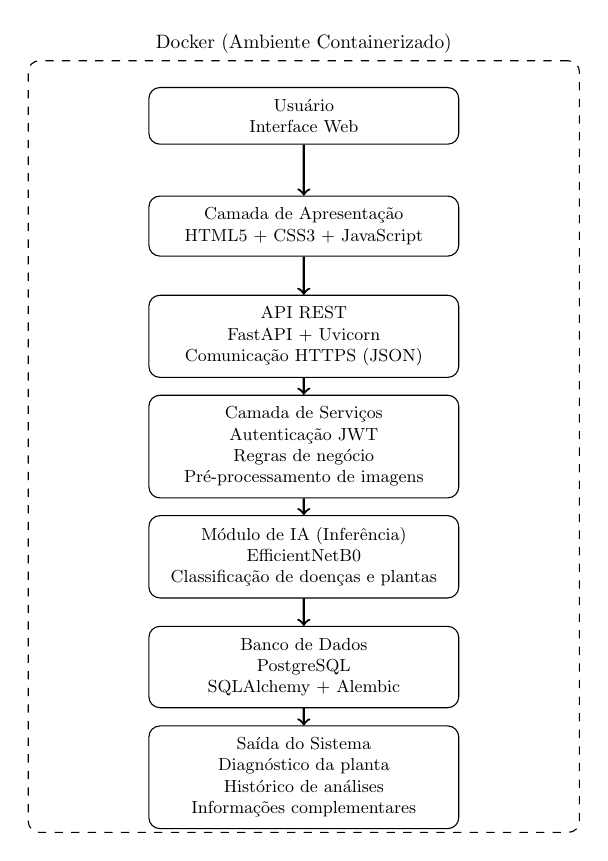
\begin{tikzpicture}[
scale=0.7,
every node/.style={transform shape},
box/.style={
draw,
rounded corners,
align=center,
font=\small,
inner sep=6pt,
text width=5.2cm
},
arrow/.style={->, thick}
]
\node[box] (usuario) at (0,0)
{Usuário\\Interface Web};
\node[box] (frontend) at (0,-2)
{Camada de Apresentação\\HTML5 + CSS3 + JavaScript};
\node[box] (api) at (0,-4)
{API REST\\FastAPI + Uvicorn\\Comunicação HTTPS (JSON)};
\node[box] (backend) at (0,-6)
{Camada de Serviços\\Autenticação JWT\\Regras de negócio\\Pré-processamento de imagens};
\node[box] (ia) at (0,-8)
{Módulo de IA (Inferência)\\EfficientNetB0\\Classificação de doenças e plantas};
\node[box] (db) at (0,-10)
{Banco de Dados\\PostgreSQL\\SQLAlchemy + Alembic};
\node[box] (saida) at (0,-12)
{Saída do Sistema\\Diagnóstico da planta\\Histórico de análises\\Informações complementares};
\draw[arrow] (usuario) -- (frontend);
\draw[arrow] (frontend) -- (api);
\draw[arrow] (api) -- (backend);
\draw[arrow] (backend) -- (ia);
\draw[arrow] (ia) -- (db);
\draw[arrow] (db) -- (saida);
\node[draw, dashed, rounded corners,
minimum width=10cm,
minimum height=14cm,
align=center,
font=\small,
label=above:Docker (Ambiente Containerizado)] at (0,-6) {};
\end{tikzpicture}
\caption{Arquitetura geral do sistema com execução containerizada em Docker.}
\label{fig:arquitetura_sistema}
\end{figure}

\subsection{Base de Dados e Ambiente Experimental}

Para o treinamento dos modelos de classificação foi utilizada a base PlantVillage \citep{ref17}, que também está disponível no
Kaggle \citep{ref7}, é  amplamente empregada em pesquisas relacionadas à detecção automática de doenças em plantas. O conjunto
de dados contém 54.309 imagens de folhas pertencentes a diferentes culturas agrícolas, incluindo amostras saudáveis e amostras
afetadas por doenças causadas por fungos, bactérias e vírus. Segundo \citep{ref17}, a construção dessa base teve 
como objetivo fornecer um repositório aberto e padronizado para o desenvolvimento de sistemas automatizados de diagnóstico 
agrícola. 

Os dados foram reorganizados em dois conjuntos independentes. O primeiro foi destinado ao treinamento de um modelo específico 
para identificação da espécie vegetal, contemplando 14 culturas presentes na base original. O segundo conjunto foi empregado 
no treinamento de um modelo especializado na identificação das doenças, considerando 38 categorias distintas. Essa estratégia 
de classificação em múltiplos estágios foi adotada com o objetivo de reduzir inconsistências entre planta e doença identificadas,
sendo compatível com abordagens hierárquicas utilizadas em sistemas de classificação agrícola \citep{ref2}.

O treinamento foi realizado na plataforma Google Colab, utilizando GPUs NVIDIA T4 para acelerar as etapas de aprendizagem. 
Os conjuntos de dados foram armazenados no Google Drive e carregados dinamicamente durante a execução dos experimentos. 
Conforme \citep{ref18}, o Google Colab disponibiliza recursos computacionais de alto desempenho, tornando-se uma alternativa 
amplamente utilizada em pesquisas envolvendo Aprendizado de Máquina e Deep Learning. 

\subsection{Treinamento e Otimização}

Os modelos de classificação foram implementados utilizando a biblioteca TensorFlow/Keras, adotando-se a arquitetura EfficientNetB0,
proposta por \citep{ref4}. Essa arquitetura emprega o conceito de escalonamento composto, permitindo balancear 
profundidade, largura e resolução da rede neural, alcançando elevado desempenho em tarefas de classificação de imagens com 
reduzido custo computacional.

Os dados foram organizados em uma estrutura de diretórios compatível com a função \textit{image\_dataset\_from\_directory}
da biblioteca TensorFlow/Keras, a qual permite o carregamento automático das imagens a partir de pastas pré-definidas. 
Foi adotada a estratégia de particionamento \textit{hold-out}, na qual o conjunto de dados tanto de plantas quanto de doenças
é dividido previamente em dois subconjuntos independentes: treinamento (\textit{train}) e validação (\textit{valid}).

Nesse contexto, a separação não é realizada dinamicamente durante a execução do código, mas sim definida na própria organização da
base de dados em diretórios distintos. Essa abordagem garante que a divisão entre os conjuntos permaneça fixa e consistente entre
diferentes execuções dos experimentos, contribuindo para a reprodutibilidade dos resultados.

A divisão adotada mantém aproximadamente 80\% das amostras para treinamento e 20\% para validação. O conjunto de treinamento é 
utilizado exclusivamente para o ajuste dos pesos da rede neural, enquanto o conjunto de validação é empregado apenas para 
monitoramento do desempenho do modelo em dados não vistos, sem influência direta no processo de otimização.

Além disso, foi definido um valor fixo de \textit{seed} (seed=42) durante o carregamento dos dados, de modo a garantir 
reprodutibilidade na ordenação e amostragem das imagens. Dessa forma, minimizam-se variações entre execuções e assegura-se 
maior confiabilidade na comparação dos resultados experimentais.

As imagens foram redimensionadas para $224 \times 224$ pixels e processadas em lotes de 16 amostras, utilizando-se a mesma 
etapa de pré-processamento empregada durante o treinamento. O desempenho foi mensurado por meio da métrica de acurácia e 
complementado pelas métricas de precisão (\textit{precision}), revocação (\textit{recall}) e F1-score, frequentemente utilizadas
em problemas de classificação multiclasse \citep{ref20}.

Com o objetivo de aumentar a variabilidade dos dados e reduzir o sobreajuste, foram aplicadas técnicas de aumento de dados 
(\textit{Data Augmentation}), incluindo rotações aleatórias e inversões horizontais das imagens. Além disso, foi utilizado o 
pré-processamento nativo da EfficientNetB0 antes do fornecimento das amostras ao modelo \citep{ref19,ref4}.

O treinamento foi realizado em duas etapas. Inicialmente, empregou-se a técnica de aprendizado por transferência
(\textit{Transfer Learning}), mantendo congeladas as camadas convolucionais previamente treinadas na base ImageNet e 
ajustando apenas as camadas responsáveis pela classificação. Posteriormente, foi realizado o processo de \textit{Fine-Tuning},
liberando parte das camadas profundas da rede para atualização dos pesos com uma taxa de aprendizado reduzida. Essas estratégias
possibilitam adaptar os conhecimentos previamente adquiridos ao domínio específico do problema, favorecendo a capacidade de 
generalização do modelo \citep{ref20,ref21}.

Para reduzir o risco de sobreajuste e tornar o treinamento mais estável, foram utilizados os mecanismos de parada antecipada 
(\textit{Early Stopping}) e ajuste adaptativo da taxa de aprendizado (\textit{ReduceLROnPlateau}) \citep{ref22}.

Ao final do processo, foram obtidos dois modelos independentes, armazenados no formato \texttt{.keras}, juntamente com arquivos 
JSON contendo os nomes das classes. Um dos modelos foi destinado à identificação da espécie vegetal e o outro à classificação das
doenças, sendo posteriormente integrados ao sistema por meio de uma estratégia de inferência em múltiplos estágios.

\begin{table}[ht]
\centering
\caption{Principais hiperparâmetros utilizados no treinamento dos modelos.}
\renewcommand{\arraystretch}{0.9} 
\setlength{\tabcolsep}{5pt}       
{\small
\begin{tabular}{lc}
\hline
Parâmetro & Valor \\
\hline
Arquitetura & EfficientNetB0 \\
Tamanho das imagens & $224 \times 224$ \\
Batch size & 16 \\
Otimizador & Adam \\
Taxa de aprendizado (fase 1) & $10^{-3}$ \\
Taxa de aprendizado (fase 2) & $10^{-5}$ \\
Função de perda & Sparse Categorical Crossentropy \\
Épocas (fase 1) & 12 \\
Épocas (fase 2) & 15 \\
Data Augmentation & Rotação e espelhamento horizontal \\
Early Stopping & Sim \\
ReduceLROnPlateau & Sim \\
Hardware & GPU NVIDIA T4 \\
Ambiente & Google Colab \\
\hline
\end{tabular}
}
\label{tab:hiperparametros}
\end{table}

\begin{figure}[ht]
\centering
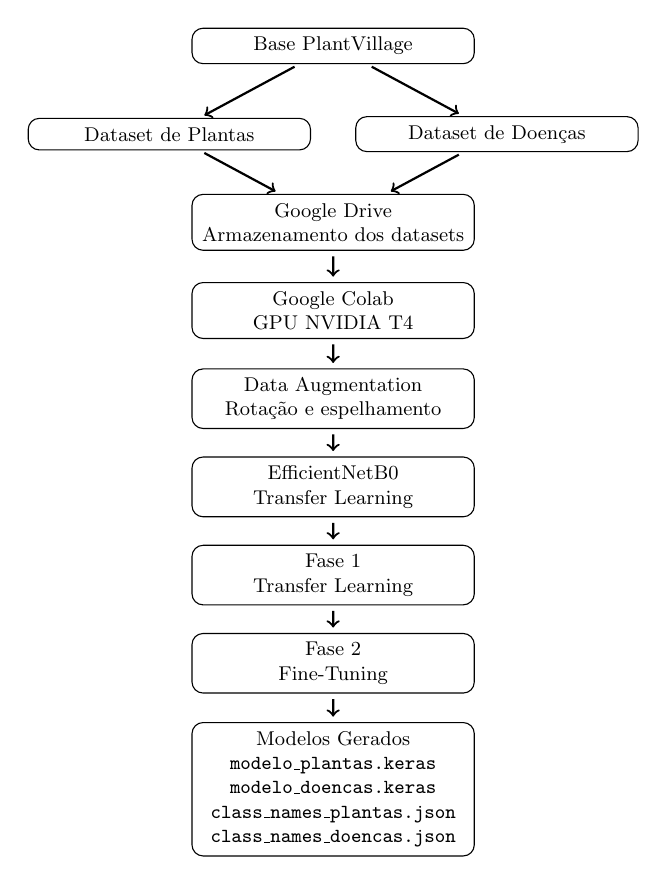
\begin{tikzpicture}[
scale=0.8,
every node/.style={transform shape},
box/.style={
draw,
rounded corners,
align=center,
font=\small,
inner sep=4pt,
text width=4.2cm
},
arrow/.style={->, thick, shorten >=2pt, shorten <=2pt}
]
\node[box] (plantvillage) at (0,0) {Base PlantVillage};
\node[box] (datasetPlantas) at (-2.6,-1.4) {Dataset de Plantas};
\node[box] (datasetDoencas) at (2.6,-1.4) {Dataset de Doenças};
\node[box] (drive) at (0,-2.8)
{Google Drive\\Armazenamento dos datasets};
\node[box] (colab) at (0,-4.2)
{Google Colab\\GPU NVIDIA T4};
\node[box] (augmentation) at (0,-5.6)
{Data Augmentation\\Rotação e espelhamento};
\node[box] (efficientnet) at (0,-7.0)
{EfficientNetB0\\Transfer Learning};
\node[box] (fase1) at (0,-8.4)
{Fase 1\\Transfer Learning};
\node[box] (fase2) at (0,-9.8)
{Fase 2\\Fine-Tuning};
\node[box] (modelos) at (0,-11.8)
{Modelos Gerados\\
\texttt{modelo\_plantas.keras}\\
\texttt{modelo\_doencas.keras}\\
\texttt{class\_names\_plantas.json}\\
\texttt{class\_names\_doencas.json}};
\draw[arrow] (plantvillage) -- (datasetPlantas);
\draw[arrow] (plantvillage) -- (datasetDoencas);
\draw[arrow] (datasetPlantas) -- (drive);
\draw[arrow] (datasetDoencas) -- (drive);
\draw[arrow] (drive) -- (colab);
\draw[arrow] (colab) -- (augmentation);
\draw[arrow] (augmentation) -- (efficientnet);
\draw[arrow] (efficientnet) -- (fase1);
\draw[arrow] (fase1) -- (fase2);
\draw[arrow] (fase2) -- ++(0,-0.6) -- (modelos);
\end{tikzpicture}
\caption{Pipeline de treinamento dos modelos de Inteligência Artificial.}
\label{fig:pipeline_ia}
\end{figure}

\subsection{Processo de Inferência e Cálculo da Confiança}

Durante a etapa de inferência, a imagem enviada pelo usuário é inicialmente submetida a um processo de pré-processamento 
compatível com a arquitetura \textit{EfficientNetB0}, incluindo redimensionamento para $224 \times 224$ pixels e normalização
por meio da função \textit{preprocess\_input} da API do TensorFlow/Keras, garantindo compatibilidade com o domínio de entrada
utilizado no treinamento.

Em seguida, a imagem é encaminhada simultaneamente para dois modelos independentes: um modelo responsável pela classificação 
da espécie vegetal e outro especializado na identificação da doença. Ambos os modelos produzem vetores de probabilidade obtidos
por meio da função \textit{softmax}, representando a distribuição de confiança entre as classes possíveis.

Para aumentar a consistência das predições, o sistema aplica uma estratégia de inferência baseada em compatibilidade biológica
entre planta e doença. As classes de doenças seguem uma estrutura hierárquica no formato \textit{Planta\_\_\_Doença}, permitindo
o mapeamento direto entre os dois modelos. A partir desse mapeamento, é estabelecida uma relação de compatibilidade entre as 
saídas dos dois modelos, permitindo avaliar a consistência biológica entre planta e doença durante o processo de seleção da 
predição final.

O processo de seleção do par planta-doença é realizado por meio de uma estratégia \textit{top-k}. São consideradas as três 
classes com maior probabilidade no modelo de plantas e as cinco classes mais prováveis no modelo de doenças. Para cada candidato,
é calculado um \textit{score} composto pela combinação ponderada das probabilidades:
\begin{equation} Score = 0{,}6 \cdot P_{doença} + 0{,}4 \cdot P_{planta} + B \end{equation}

em que $B$ representa um bônus adicional de consistência, aplicado quando a planta associada à doença candidata está entre as 
três classes mais prováveis do modelo de plantas.

O par final é definido como aquele que apresenta o maior \textit{score} entre todas as combinações avaliadas. Caso nenhum par 
compatível seja encontrado, o sistema recorre a uma estratégia de \textit{fallback} baseada na maior probabilidade global do 
modelo de doenças, associada à melhor correspondência disponível no modelo de plantas.

Casos específicos são tratados por regras adaptativas. Para culturas com baixa representatividade no conjunto de dados, como
\textit{Blueberry}, \textit{Raspberry}, \textit{Orange} e \textit{Cherry}, a confiança final é obtida diretamente a partir 
da probabilidade produzida pelo modelo de doenças, reduzindo a influência do classificador de plantas. Já para a cultura
\textit{Tomato}, são aplicados ajustes adicionais baseados na distribuição das probabilidades, com análise de múltiplas 
classes candidatas, visando reduzir ambiguidades entre doenças visualmente semelhantes.

Além disso, heurísticas específicas são utilizadas para corrigir classificações instáveis, como o caso de predições incorretas 
de \textit{healthy} quando há forte evidência de outras doenças no vetor de saída.

Após a definição do par planta-doença, o nome da doença é normalizado e o resultado final é representado no formato
\textit{planta\_\_\_doença}. A confiança final da predição é estimada de acordo com a disponibilidade de dados para cada cultura.

(i) Para culturas com poucos dados, utiliza-se diretamente a probabilidade do modelo de doenças;

(ii) Para as demais culturas, aplica-se uma combinação ponderada entre os dois modelos:
\begin{equation} Confiança_{final} = 0{,}65 \cdot P_{doença} + 0{,}35 \cdot P_{planta} \end{equation}

Essa abordagem híbrida permite integrar informações complementares dos dois classificadores, aumentando a robustez do sistema,
reduzindo inconsistências entre saídas independentes e melhorando a confiabilidade das predições finais.

\begin{figure}[ht]
\centering
\begin{tikzpicture}[
scale=0.65,
every node/.style={transform shape},
box/.style={
draw,
rounded corners,
align=center,
font=\footnotesize,
inner sep=4pt,
text width=3.8cm
},
arrow/.style={->, thick}
]
\node[box] (input) at (0,0)
{Imagem enviada pelo usuário};
\node[box] (preproc) at (0,-1.8)
{Pré-processamento\\
Redimensionamento ($224\times224$)\\
Normalização};
\node[box] (plant) at (-3.2,-4.5)
{Modelo de Planta\\
EfficientNetB0\\
Probabilidades das espécies};
\node[box] (disease) at (3.2,-4.5)
{Modelo de Doença\\
EfficientNetB0\\
Probabilidades das doenças};
\node[box,text width=5.8cm] (selection) at (0,-7.5)
{Seleção do par planta-doença\\
Top-3 plantas + Top-5 doenças\\
Score = $0,6P_{doença}+0,4P_{planta}+B$};
\node[box,text width=5.8cm] (rules) at (0,-10)
{Regras adaptativas\\
Compatibilidade biológica\\
Correções para Tomato e falso healthy\\
Fallback quando necessário};
\node[box,text width=5.8cm] (confidence) at (0,-12.5)
{Cálculo da confiança final\\
$\mathrm{Conf}=0,65P_{doença}+0,35P_{planta}$\\
ou apenas $P_{doença}$ para plantas com poucos dados};
\node[box] (output) at (0,-15)
{Resultado final\\
Planta identificada\\
Doença identificada\\
Nível de confiança};
\draw[arrow] (input) -- (preproc);
\draw[arrow] (preproc) -- (plant);
\draw[arrow] (preproc) -- (disease);
\draw[arrow] (plant) -- (selection);
\draw[arrow] (disease) -- (selection);
\draw[arrow] (selection) -- (rules);
\draw[arrow] (rules) -- (confidence);
\draw[arrow] (confidence) -- (output);
\end{tikzpicture}
\caption{Fluxo do processo de inferência e cálculo da confiança do sistema proposto.}
\label{fig:fluxo_inferencia}
\end{figure}

\subsection{Integração com Modelos de Linguagem}

Além do processo de classificação das doenças, foi implementado um módulo de geração automática de descrições textuais complementares
associadas aos resultados obtidos pelo sistema. Esse módulo tem como objetivo fornecer informações educativas sobre a planta e a 
possível condição fitossanitária identificada, auxiliando o usuário na compreensão do diagnóstico produzido pelos modelos de 
Inteligência Artificial.

Para essa finalidade, foram utilizados modelos de linguagem acessados por meio de uma API de terceiros (OpenRouter), que atua como 
intermediador para a utilização de modelos de linguagem de grande porte. Essa abordagem permite a geração de textos explicativos em 
linguagem natural, sem a necessidade de gerenciamento direto da infraestrutura do modelo.

As respostas geradas são estruturadas de forma a apresentar descrições gerais sobre a doença detectada, incluindo características 
visuais comuns, possíveis causas biológicas e condições ambientais associadas ao seu desenvolvimento.

É importante destacar que o sistema não realiza a prescrição de tratamentos de intervenção química de agrotóxicos.
Essa decisão foi adotada para evitar riscos decorrentes de possíveis erros de classificação, uma vez que diagnósticos incorretos 
poderiam levar a ações inadequadas e impactos ambientais indesejados.

Dessa forma, o módulo é restrito à geração de informações de caráter educativo e informativo, não devendo ser interpretado como 
substituto de orientação técnica especializada. Conforme descrito por \citep{ref23}, modelos de linguagem de grande porte apresentam 
elevada capacidade de geração de texto contextualizado, sendo amplamente utilizados em aplicações de apoio à comunicação e 
disseminação de conhecimento.

\section{Resultados e Discussões}
\label{sec:Resultados e Discussões}
\subsection{Avaliação dos Modelos}

A avaliação dos modelos foi realizada utilizando os subconjuntos de validação disponibilizados na organização da base 
PlantVillage, correspondentes da divisão fixa do tipo Hold-out, na qual aproximadamente 80\% das imagens são utilizadas para
treinamento e cerca de 20\% das imagens para validação. O desempenho dos classificadores foi analisado a partir das previsões obtidas sobre
esse conjunto, permitindo verificar a capacidade de generalização dos modelos para amostras não utilizadas durante o treinamento.

Para a classificação das espécies vegetais, o modelo baseado na arquitetura EfficientNetB0 apresentou elevada capacidade de 
generalização, alcançando acurácia superior a 96\% sobre o conjunto de validação. De forma semelhante, o modelo destinado à 
identificação das doenças atingiu acurácia próxima de 98\% evidenciando a eficiência da estratégia baseada em aprendizado por
transferência e ajuste fino das camadas mais profundas da rede.

Além da acurácia global, foram analisadas as matrizes de confusão dos modelos, permitindo identificar as principais ocorrências
de classificações incorretas. Observou-se que a maior parte dos erros concentrou-se entre classes que apresentam características
visuais semelhantes, especialmente em doenças foliares com sintomas próximos ou em estágios iniciais de desenvolvimento. 
Esse comportamento é consistente com resultados encontrados na literatura sobre classificação automática de doenças em 
plantas baseada em Visão Computacional \citep{ref2}.

Os resultados obtidos indicam que a utilização da EfficientNetB0 associada às técnicas de \textit{Transfer Learning}, 
\textit{Fine-Tuning}, aumento de dados e mecanismos de regularização contribuiu para a obtenção de modelos com elevada 
capacidade de discriminação entre as classes, tornando-os adequados para integração à plataforma desenvolvida.

\section{Conclusão}

Excepteur sint occaecat cupidatat non proident, sunt in culpa qui officia deserunt mollit anim id est laborum. Lorem ipsum dolor sit amet, consectetur adipiscing elit, sed do eiusmod tempor incididunt ut labore et dolore magna aliqua. Ut enim ad minim veniam, quis nostrud exercitation ullamco laboris nisi ut aliquip ex ea commodo consequat. Duis aute irure dolor in reprehenderit in voluptate velit esse cillum dolore eu fugiat nulla pariatur. 

Lorem ipsum dolor sit amet, consectetur adipiscing elit, sed do eiusmod tempor incididunt ut labore et dolore magna aliqua. Ut enim ad minim veniam, quis nostrud exercitation ullamco laboris nisi ut aliquip ex ea commodo consequat. Excepteur sint occaecat cupidatat non proident, sunt in culpa qui officia deserunt mollit anim id est laborum. Lorem ipsum dolor sit amet, consectetur adipiscing elit, sed do eiusmod tempor incididunt ut labore et dolore magna aliqua. Ut enim ad minim veniam, quis nostrud exercitation ullamco laboris nisi ut aliquip ex ea commodo consequat. Duis aute irure dolor in reprehenderit in voluptate velit esse cillum dolore eu fugiat nulla pariatur. Excepteur sint occaecat cupidatat non proident, sunt in culpa qui officia deserunt mollit anim id est laborum \citep{ref5}.


\begin{declarations}

\begin{acknowledgements}
ESTA DECLARAÇÃO É OPCIONAL. Este é um texto de agradecimentos com várias linhas. Lorem ipsum dolor sit amet, consectetur adipiscing elit, sed do eiusmod tempor incididunt ut labore et dolore magna aliqua. Ut enim ad minim veniam, quis nostrud exercitation ullamco laboris nisi ut aliquip ex ea commodo consequat.
\end{acknowledgements}

\begin{contributions}
ESTA DECLARAÇÃO É OBRIGATÓRIA. Sugerimos que os autores descrevam sua contribuição usando a Taxonomia CRediT (\href{https://credit.niso.org/}{https://credit.niso.org/}) como neste exemplo: JV contribuiu para a concepção deste estudo. CB, RP e CM realizaram os experimentos. JV é o principal contribuidor e escritor deste manuscrito. Todos os autores leram e aprovaram o manuscrito final. 
\end{contributions}

\begin{interests}
ESTA DECLARAÇÃO É OBRIGATÓRIA. Se não houver conflitos de interesse, os autores devem declarar: ``Os autores declaram que não têm nenhum conflito de interesses''. Caso contrário, a declaração deve ser: ``Os autores declaram que têm os seguintes conflito de interesses: lorem ipsum dolor sit amet, consectetur adipiscing elit.''
\end{interests}

\begin{materials}
ESTA DECLARAÇÃO É OBRIGATÓRIA. 
  Se os autores estiverem disponibilizando seus dados e/ou códigos
  abertamente, a declaração deve ser: ``Os conjuntos de dados (e/ou
  softwares) gerados e/ou analisados durante o estudo atual estão
  disponíveis em \ldots''. Caso contrário, a declaração deve ser: ``Os
  conjuntos de dados (e/ou softwares) gerados e/ou analisados durante
  o estudo atual serão feitos mediante solicitação''.
\end{materials}

\begin{furtherinformation}
ESTA DECLARAÇÃO É DESEJÁVEL. Informações adicionais relevantes, como, por exemplo, a aprovação em comitê de ética ou o uso de ferramentas de IA generativa no desenvolvimento do artigo. Essa declaração é opcional, se não houver nada a ser acrescentado, pode ser deixada em branco
\end{furtherinformation}
\end{declarations}



\bibliographystyle{apalike-sol}
\bibliography{refs}

\end{document}

Se os autores estiverem disponibilizando seus dados e/ou códigos abertamente,
 a declaração deve ser: ``Os conjuntos de dados (e/ou softwares)
 gerados e/ou analisados ​​durante o estudo atual estão disponíveis em
 lorem ipsum dolor sit amet''. Caso contrário, a declaração deve ser:
 ``Os conjuntos de dados (e/ou softwares) gerados e/ou analisados durante o estudo atual serão
  feitos mediante solicitação''.
